% goldie-and-draghino.tex
% "Goldie and Draghino: Two Dragons, Two Cities"
% A 24-page illustrated children's book (ages 6-10)
%
% Compile with: pdflatex goldie-and-draghino.tex (run twice)
%            or: lualatex goldie-and-draghino.tex (run twice)
%
% Place AI-generated images as page-01.png through page-24.png
% in the images/ subdirectory. See image-prompts.md for prompts.

\documentclass[14pt, letterpaper, oneside]{extarticle}

\usepackage[
  paperwidth=8.5in,
  paperheight=8.5in,
  left=0.6in,
  right=0.6in,
  top=0.5in,
  bottom=0.7in
]{geometry}

\usepackage{graphicx}
\usepackage{xcolor}
\usepackage{microtype}
\usepackage{avant}          % TeX Gyre Adventor (geometric sans-serif)
\renewcommand{\familydefault}{\sfdefault}

% Point graphicx to the images/ subdirectory
\graphicspath{{images/}}

% No page numbers
\pagestyle{empty}

% Paragraph settings for story text
\setlength{\parindent}{0pt}
\setlength{\parskip}{0.4em}

%% ========================================================
%% PAGE LAYOUT MACROS
%% ========================================================

% Layout A: Full-page illustration with text below
% #1 = image filename (without extension)
% #2 = Story text
\newcommand{\storypage}[2]{%
  \clearpage
  \vspace*{-0.2in}
  \begin{center}
    \IfFileExists{images/#1.png}{%
      \includegraphics[width=\textwidth, height=4.5in, keepaspectratio]{#1}%
    }{%
      % Placeholder when image is not yet available
      \fcolorbox{gray}{gray!10}{%
        \parbox[c][4.5in][c]{\dimexpr\textwidth-2\fboxsep-2\fboxrule}{%
          \centering\large\color{gray}%
          [Illustration: #1.png]\\[0.3em]
          \small See image-prompts.md for generation prompt%
        }%
      }%
    }
  \end{center}
  \vspace{-0.1in}
  \begin{center}
    \parbox{0.9\textwidth}{%
      \normalsize #2%
    }
  \end{center}
  \vfill
}

% Layout B: Top illustration (smaller), bottom text
% #1 = image filename (without extension)
% #2 = Story text
\newcommand{\storypageB}[2]{%
  \clearpage
  \vspace*{0.05in}
  \begin{center}
    \IfFileExists{images/#1.png}{%
      \includegraphics[width=0.85\textwidth, height=3.5in, keepaspectratio]{#1}%
    }{%
      % Placeholder when image is not yet available
      \fcolorbox{gray}{gray!10}{%
        \parbox[c][3.5in][c]{\dimexpr0.85\textwidth-2\fboxsep-2\fboxrule}{%
          \centering\large\color{gray}%
          [Illustration: #1.png]\\[0.3em]
          \small See image-prompts.md for generation prompt%
        }%
      }%
    }
  \end{center}
  \vspace{0.1in}
  \begin{center}
    \parbox{0.9\textwidth}{%
      \normalsize #2%
    }
  \end{center}
  \vfill
}

%% ========================================================
\begin{document}
%% ========================================================

%% --------------------------------------------------------
%% PAGE 1 — TITLE PAGE
%% --------------------------------------------------------
\begin{center}
\vspace*{0.5in}

{\fontsize{28}{34}\selectfont\bfseries
Goldie and Draghino}

\vspace{0.15in}

{\fontsize{16}{20}\selectfont\itshape
Two Dragons, Two Cities}

\vspace{0.4in}

\IfFileExists{images/page-01.png}{%
  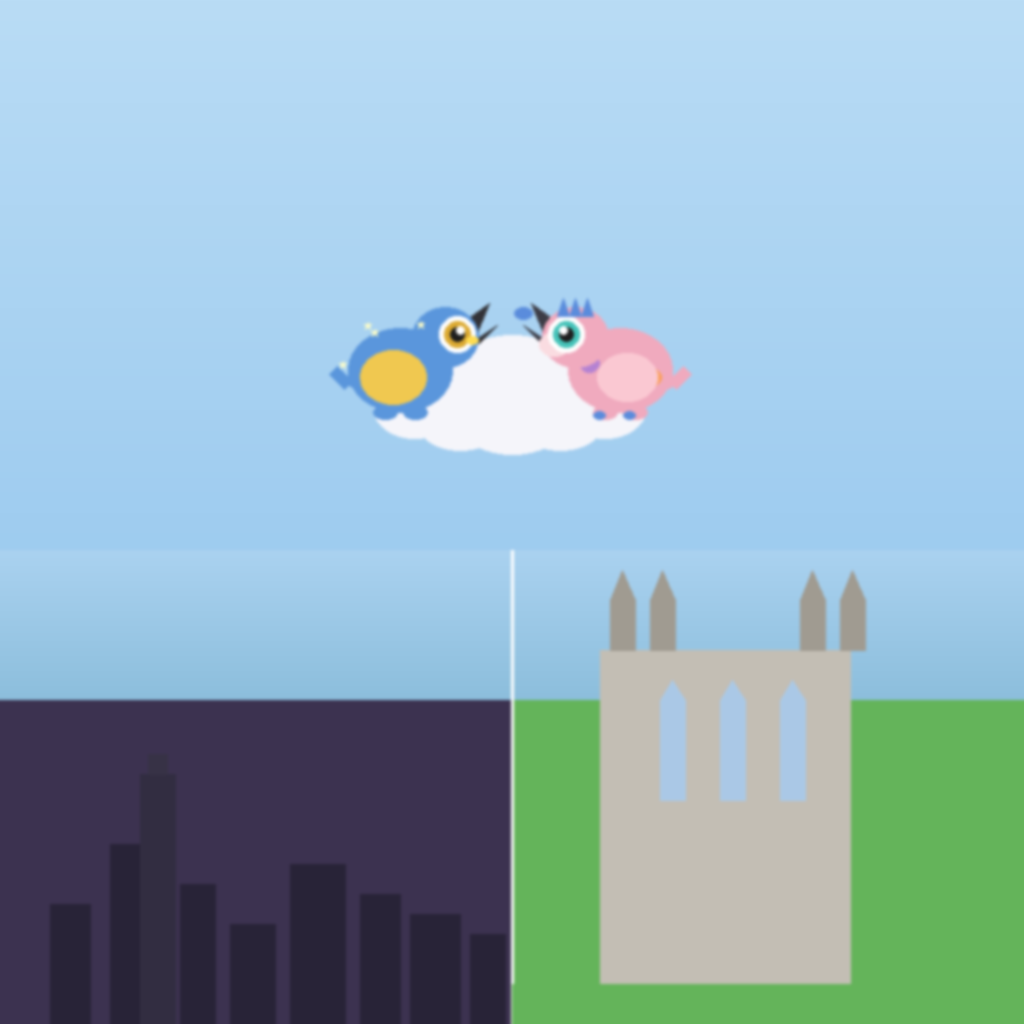
\includegraphics[width=0.85\textwidth, height=4.0in, keepaspectratio]{page-01}%
}{%
  \fcolorbox{gray}{gray!10}{%
    \parbox[c][4.0in][c]{0.8\textwidth}{%
      \centering\large\color{gray}%
      [Title illustration: page-01.png]\\[0.3em]
      \small Both dragons on a cloud, Rochester/Cambridge below%
    }%
  }%
}

\vspace{0.5in}

{\large\itshape A story about friendship, adventure,\\ and finding home.}

\end{center}
\vfill

%% --------------------------------------------------------
%% PAGE 2 — MEET GOLDIE
%% --------------------------------------------------------
\storypageB{page-02}{
In a cozy cave overlooking the Genesee River in Rochester, New York, lived a sparkly blue dragon named Goldie. Her scales shimmered like the sky on a summer day, and her golden belly glowed like the sunrise over Lake Ontario.

She had big, bright amber eyes that noticed everything --- every falling leaf, every ripple in the river, every star that came out at night.
}

%% --------------------------------------------------------
%% PAGE 3 — MEET DRAGHINO
%% --------------------------------------------------------
\storypageB{page-03}{
Next door, in a garden bursting with every colour you could imagine, lived Draghino --- a dragon painted in all the shades of the rainbow.

Pink and purple and yellow and green spots covered Draghino's chubby round body. Bright teal eyes sparkled with curiosity, and three little blue horns sat proudly on top. Draghino thought every day was an adventure waiting to happen.
}

%% --------------------------------------------------------
%% PAGE 4 — BEST FRIENDS (Genesee River)
%% --------------------------------------------------------
\storypage{page-04}{
Goldie and Draghino were the very best of friends. Every morning they met by the Genesee River and planned their day together. In autumn, the trees along the banks turned orange and red, and the two dragons would race through the falling leaves, laughing until their bellies ached.
}

%% --------------------------------------------------------
%% PAGE 5 — HIGH FALLS
%% --------------------------------------------------------
\storypage{page-05}{
Their favourite spot was High Falls, where the Genesee River thundered over a cliff and crashed into a pool of swirling mist far below.

``I bet I could fly right through that mist!'' said Goldie.

``I bet you would get \emph{very} wet,'' laughed Draghino.
}

%% --------------------------------------------------------
%% PAGE 6 — STRONG MUSEUM
%% --------------------------------------------------------
\storypageB{page-06}{
On rainy days they visited the Strong Museum --- the National Museum of Play! They played with every exhibit they could find: giant board games, rooms full of toys, and video games from long, long ago.

``This is the best museum in the whole world,'' said Draghino, bouncing on a giant rubber ball. Goldie agreed, though she preferred the butterfly garden upstairs.
}

%% --------------------------------------------------------
%% PAGE 7 — ROCHESTER WINTER
%% --------------------------------------------------------
\storypage{page-07}{
When winter came, Rochester turned white. Snow piled up on every roof and every branch, and the two friends built snow-dragons in the park.

Goldie's golden tummy made an excellent sled for sliding down the hills. ``Wheeeee!'' she cried, while Draghino tumbled along behind, leaving a rainbow trail in the snow.
}

%% --------------------------------------------------------
%% PAGE 8 — GARBAGE PLATE
%% --------------------------------------------------------
\storypageB{page-08}{
And when they were hungry, there was only one thing to eat: a \textbf{garbage plate}! That is what people in Rochester call their most famous meal --- a giant plate piled high with macaroni salad, fries, hot dogs, and plenty of hot sauce.

``More mac salad!'' cried Draghino.

``More hot sauce!'' cheered Goldie.

They always ate every last bite.
}

%% --------------------------------------------------------
%% PAGE 9 — THE LETTER
%% --------------------------------------------------------
\storypageB{page-09}{
One morning, a letter arrived for Goldie. It had a fancy red seal and came from very far away.

``It is from Cambridge,'' said Goldie, her golden eyes wide with wonder. ``In \emph{England}. They have heard about my research on sparkly rocks, and they want me to come and study there!''

Draghino looked at the letter, then looked at Goldie, then looked at the letter again.
}

%% --------------------------------------------------------
%% PAGE 10 — THE DILEMMA (Rochester skyline at sunset)
%% --------------------------------------------------------
\storypage{page-10}{
That evening, they climbed the highest hill and watched the sun set behind the Rochester skyline. The Kodak Tower stood tall and proud against the orange sky.

``But I cannot leave you behind,'' said Goldie quietly.

Draghino smiled their biggest smile. ``Who said anything about leaving me behind? Where you go, I go. That is what best friends do.''
}

%% --------------------------------------------------------
%% PAGE 11 — PACKING
%% --------------------------------------------------------
\storypageB{page-11}{
They packed everything they could carry. Goldie packed her books and her sparkly rock collection. Draghino insisted on bringing twelve jars of hot sauce.

``You cannot get a proper garbage plate in England,'' Draghino said wisely.

``I do not think you can get one \emph{anywhere} except Rochester,'' said Goldie.

``Exactly my point,'' said Draghino, sitting firmly on an overstuffed suitcase.
}

%% --------------------------------------------------------
%% PAGE 12 — SAYING GOODBYE
%% --------------------------------------------------------
\storypage{page-12}{
``Goodbye, Rochester,'' they said together, looking down at the city growing smaller and smaller beneath them. ``Thank you for the falls and the snow and the plates.''

The city twinkled below them like a box of stars, and the Genesee River wound through it like a silver ribbon.
}

%% --------------------------------------------------------
%% PAGE 13 — OVER THE ATLANTIC (DAY)
%% --------------------------------------------------------
\storypage{page-13}{
They flew east, over the wide Atlantic Ocean. The water stretched out in every direction --- blue and green and silver, sparkling in the sunlight.

Far below, a tiny ship sailed across the waves. ``Do you think they can see us?'' asked Draghino.

``I hope so,'' said Goldie. ``It is not every day you see two dragons flying to England.''
}

%% --------------------------------------------------------
%% PAGE 14 — OVER THE ATLANTIC (NIGHT)
%% --------------------------------------------------------
\storypageB{page-14}{
They flew through the night. A thousand stars hung above them, and the moon painted a silver path across the dark water below.

Draghino yawned a tremendous yawn. ``Are we there yet?''

``Almost,'' said Goldie, though she was not entirely sure. The ocean was very, very big.

``Wake me when we get there,'' mumbled Draghino, somehow falling asleep while still flying.
}

%% --------------------------------------------------------
%% PAGE 15 — FIRST SIGHT OF ENGLAND
%% --------------------------------------------------------
\storypage{page-15}{
As the sun rose, green fields appeared below them --- tiny squares of emerald and gold stitched together like a quilt. Hedgerows drew neat lines between them, and a river wound through the patchwork like a thread of blue silk.

``That is England!'' cried Goldie.

Draghino opened one eye, looked down, and opened the other eye very wide indeed. ``It is so \emph{green},'' Draghino whispered.
}

%% --------------------------------------------------------
%% PAGE 16 — ARRIVING IN CAMBRIDGE (King's College)
%% --------------------------------------------------------
\storypageB{page-16}{
They landed softly on a wide green lawn. Before them stood the most beautiful building they had ever seen --- King's College Chapel, with its tall stone towers reaching toward the clouds.

``Look at those windows,'' said Goldie. ``They must be a hundred feet tall.''

``Look at that grass,'' said Draghino. ``It is the greenest grass I have ever seen. Can we sit on it?''

A small sign said: \emph{Please keep off the grass.}

``I suppose not,'' sighed Draghino.
}

%% --------------------------------------------------------
%% PAGE 17 — PUNTING ON THE CAM
%% --------------------------------------------------------
\storypage{page-17}{
They tried punting on the River Cam. This meant standing in a long, flat boat and pushing a pole against the river bottom to move along. It looked easy. It was not easy.

Goldie pushed the pole. The boat spun in a circle. Draghino grabbed the edge and laughed so hard they nearly fell in.

``I think we need more practice,'' said Goldie, as the punt drifted gently into a willow tree.

A duck watched them with what looked a lot like disapproval.
}

%% --------------------------------------------------------
%% PAGE 18 — MATHEMATICAL BRIDGE
%% --------------------------------------------------------
\storypageB{page-18}{
At Queens' College, they found the famous Mathematical Bridge --- a wooden bridge that curved gracefully over the river, its beams arranged in a clever pattern.

``They say this bridge was designed with brilliant mathematics!'' said Goldie, reading a sign with great excitement.

``Just like how I keep my spots on,'' said Draghino. ``Pure magic and mathematics.''

``That is not how spots work,'' said Goldie.

``Prove it,'' said Draghino.

Goldie could not, in fact, prove it.
}

%% --------------------------------------------------------
%% PAGE 19 — MARKET SQUARE
%% --------------------------------------------------------
\storypage{page-19}{
At the Market Square in the centre of town, they found stalls selling cakes and scarves and old books and bunches of flowers.

Draghino found a scarf striped with every colour of the rainbow. ``It matches me!'' Draghino said happily, wrapping it around three times.

Goldie bought a very old book about sparkly rocks. ``This book is four hundred years old,'' she whispered.

``Is it older than the Mathematical Bridge?'' asked Draghino.

``Much older,'' said Goldie.
}

%% --------------------------------------------------------
%% PAGE 20 — MAKING FRIENDS
%% --------------------------------------------------------
\storypageB{page-20}{
They met hedgehogs and foxes and robins who all lived in the college gardens.

``Welcome to Cambridge,'' said a very small hedgehog, peering up at them with shiny black eyes. ``We have been hoping for some dragons.''

``You have?'' said Goldie, surprised.

``Oh yes,'' said the hedgehog. ``Nobody else can reach the high branches to shake down the acorns.''

Draghino immediately shook the nearest tree. Acorns rained down like hailstones.
}

%% --------------------------------------------------------
%% PAGE 21 — MISSING ROCHESTER
%% --------------------------------------------------------
\storypage{page-21}{
Sometimes, on rainy afternoons, they missed Rochester.

They missed the thunder of High Falls and the crunch of snow under their feet. They missed the Strong Museum and the taste of a garbage plate with extra hot sauce.

``Do you think Rochester misses us?'' asked Draghino, pressing a pink nose against the glass.

``I am sure it does,'' said Goldie. ``But I also think it is happy that we are having an adventure.''
}

%% --------------------------------------------------------
%% PAGE 22 — HOME IS WHO YOU'RE WITH
%% --------------------------------------------------------
\storypageB{page-22}{
One afternoon, sitting on a bench in a sunny Cambridge park, Goldie said something very wise.

``I think,'' she said slowly, ``that home is not a place you can find on a map. Home is who you are with.''

Draghino thought about this for a long moment.

``Then I am always home,'' said Draghino, ``because I am always with you.''

Goldie's golden belly glowed a little brighter, which is what happens when a dragon is very, very happy.
}

%% --------------------------------------------------------
%% PAGE 23 — CAMBRIDGE AT NIGHT
%% --------------------------------------------------------
\storypage{page-23}{
That night, they sat on a rooftop and watched the stars come out above Cambridge. The old city glowed golden below them, and the great chapel windows shone with warm light.

``You know,'' said Draghino, ``Rochester and Cambridge are not really so different. They both have rivers. They both have beautiful buildings. And they both have us.''

``And somewhere,'' said Goldie, looking up at the stars, ``Rochester is looking at this same moon.''
}

%% --------------------------------------------------------
%% PAGE 24 — THE END
%% --------------------------------------------------------
\storypageB{page-24}{
And so two dragons from Rochester found a new home in Cambridge --- but they carried their old home with them, right in their hearts.

On the wall hung a Rochester pennant and a Cambridge scarf, side by side. On the shelf sat twelve jars of hot sauce (well, eleven --- they had already used one).

And in a cozy pile of blankets, two best friends curled up together and dreamed of rivers and waterfalls and garbage plates and Gothic spires and all the adventures still to come.

\begin{center}
\vspace{0.3in}
{\fontsize{20}{24}\selectfont\bfseries The End}
\end{center}
}

%% ========================================================
\end{document}
%% ========================================================
